\documentclass{beamer}
\usepackage[utf8]{inputenc}
\usepackage{xmpmulti}
\usepackage{listings}
\usepackage{booktabs}
\usepackage{nicefrac}
\usepackage{amssymb}
\usepackage{amsmath}
\usepackage{bm}
\usepackage{enumitem}
\usepackage{hyperref}
\usepackage[export]{adjustbox}
\usepackage{svg}

\usetheme{Madrid}
\definecolor{mlpblue}{rgb}{0.1, 0.14, 0.24}

\useoutertheme{infolines} % Alternatively: miniframes, infolines, split
\useinnertheme{circles}
\usecolortheme[named=mlpblue]{structure}

\lstset{basicstyle=\footnotesize\ttfamily,breaklines=true}

%------------------------------------------------------------
%This block of code defines the information to appear in the
%Title page
\title[Neural Tangent Kernel]{Neural Tangent Kernel}

\subtitle{Comprehending Convergence \& Generalization in Neural Networks\thanks{\href{https://arxiv.org/abs/1806.07572}{Jacot, Gabriel, Hongler.~[NIPS 2018]}}}

\author[Machine Learning @ Purdue] % optional
{J.~Setpal} 

\date{March 6, 2025}

\titlegraphic{
\includegraphics[width=7cm]{../shared/logo-long.pdf}}

%End of title page configuration block
%------------------------------------------------------------

%The next block of commands puts the table of contents at the 
%beginning of each section and highlights the current section:

\AtBeginSection[]
{
  \begin{frame}
    \frametitle{Outline}
    \tableofcontents[currentsection]
  \end{frame}
}
% ------------------------------------------------------------


\begin{document}

\frame{\titlepage}


%---------------------------------------------------------
% This block of code is for the table of contents after
% the title page
\begin{frame}
\frametitle{Outline}
\tableofcontents
\end{frame}
%---------------------------------------------------------

\section{Background \& Intuition}

\begin{frame}{Problem Setting}
	Given network $f_\theta: \mathbb{R}^d \rightarrow \mathbb{R}$, we have two distinctive regimes: \\
	Underparameterized Learning: $\bm{n \geq p}, \quad \theta \in \mathbb{R}^p, \quad \mathcal{D} = \{(x_i, y_i)\}^n_{i=1}$ \\
	Overparameterized Learning: $\bm{p \geq n}, \quad \theta \in \mathbb{R}^p, \quad \mathcal{D} = \{(x_i, y_i)\}^n_{i=1}$ \pause \newline \\

	Either way, we optimize $\theta$ to minimize an empirical loss (here, quadratic):
	\begin{gather}
		\mathcal{L}(\theta, \mathcal{D}) = \frac{1}{n} \sum^n_{i=1} \ell(f_\theta(x_i), y_i) = \frac{1}{n} \| f_\theta(\bm{x}) - \bm{y} \|^2_2
	\end{gather} \pause

	\textbf{Q}: Why does overparameterized learning generalize? \pause \\
	\textbf{A}: NTK's approach:
	\begin{enumerate}[label=\alph*.]
		\item Construct an analogy to a simpler paradigm (kernel methods). \pause
		\item Prove the analogy actually holds for sufficiently wide networks. \pause
		\item Use the analysis from the kernel method to understand training dynamics of the neural network.
	\end{enumerate}
\end{frame}

\begin{frame}{Pre-Requisite $\nicefrac{1}{3}$ -- Taylor Series}
	We can approximate function $g$ using a polynomial via the Taylor Series:
	\begin{gather}
		P_a(x) = \sum^\infty_{i=0} \frac{g^{(n)}(a)}{n!}(x - a)^{n}
	\end{gather} \pause
	The first-order Taylor Expansion is a linear approximation of the function:
	\begin{gather}
		P_a(x) = g(a) + g'(a)(x - a)
	\end{gather} \pause
	We will use the first-order approximation to model \textbf{training dynamics in neural networks}.
\end{frame}

\begin{frame}{Pre-Requisite $\nicefrac{2}{3}$ -- Operator Norm}
	The operator norm of matrix $A$ is the maximum amount of stretching that $A$ can do to arbitrary vector $x$:
	\begin{gather}
		A \in \mathbb{R}^{m \times n}, \quad x \in \mathbb{R}^n \\
		\|A\|_{\text{op}} = \max_{x \in \mathbb{R}^n} \frac{\| Ax \|_p}{\| x \|_q}
	\end{gather}
	Usually $p = q = 2$.
\end{frame}

\begin{frame}{Pre-Requisite $\nicefrac{3}{3}$ -- Kernel Methods}
	$K: \mathbb{R}^m \times \mathbb{R}^m \rightarrow \mathbb{R}$ is a kernel if $\exists\phi: \mathcal{X} \rightarrow \mathcal{H}$ s.t:
	\begin{gather}
		K(x, x') = \phi(x)^T \phi(x') = \langle \phi(x), \phi(x') \rangle
	\end{gather}
	Any PSD matrix defines a kernel. \pause \newline \\

	A kernel methods are \textbf{instance-based} learners, instead of learning parameters over input features, we learn parameters over data-pairs, and interpolate using the kernel function to predict for the unseen sample. \pause \newline 

	As an example:
	\begin{gather}
		\hat{y} = \textbf{sgn} \sum^n_{i=1} w_i y_i k(x, x')
	\end{gather}
\end{frame}

% \begin{frame}{Kernel Gradient}
% 	Consider $K$ approximated by a choice of $P$ random function sampled iid from $\mathcal{F}$
% 	\begin{gather}
% 		\mathbb{E}[f_k(x), f_k(x')] =
% 	\end{gather}
% 	training the wide neural network and kernel methods: gradient descent in the infinite-width limit is fully equivalent to kernel gradient descent with the NTK
% \end{frame}

\section{Neural Tangent Kernel}

\begin{frame}{Neural Network Setup}
	We have fully-connected network $f_\theta$ with $n_0, \ldots, n_L$ neurons in each layer, activation function $\sigma: \mathbb{R} \rightarrow \mathbb{R}$ with pre-activations $\tilde{\alpha}$ and activations $\alpha$ defined recursively as follows:
	\begin{align}
		\alpha^{(0)}(x;~\theta) &= x \\
		\tilde{\alpha}^{(\ell + 1)}(x;~\theta) &= \frac{1}{\sqrt{n_\ell}} W^{(\ell)} \alpha^{(\ell)}(x; \theta) + \beta b^{(\ell)} \\
		\alpha^{(\ell)}(x;~\theta) &=  \sigma (\tilde{\alpha}^{(\ell)}(x; \theta))
	\end{align}
	A \textbf{realization function} $F^{(L)}: \mathbb{R}^p \rightarrow \mathcal{F}$ maps parameters to a function. \pause \newline \\
	\vspace{-.7em}
	At initialization, $\theta \sim \mathcal{N}(0, I_p)$. \pause As a result at initialization, our network is equivalent to a gaussian process. \pause

	\begin{block}{\bf Aside}
		Factors $\nicefrac{1}{\sqrt{n_\ell}},~\beta$ scale gradients \& enable consistent aymptotic behavior.
	\end{block}
\end{frame}

\begin{frame}{Studying Convergence in Function Space}
	Notice that quadratic loss\footnote{also most others} is \textbf{convex w.r.t.~function space} but often \textbf{non-convex w.r.t.~parameter space}.
	\begin{align}
		C&: \mathcal{F} \rightarrow \mathbb{R} & \text{Convex~ :D} \\ 
		C \circ F^{(L)}&: \mathbb{R}^p \rightarrow \mathbb{R} & \text{Highly Non-Convex~ D:}
	\end{align} \pause
	Now, if we could analyze training in the convex setting, we can obtain meaningful insight about convergence of these networks. \pause \\
	\textbf{Q${}_1$:} How can we do that? \\
	\textbf{A${}_1$:} By constructing a first-order approximation of training dynamics. \pause \newline \\

	\textbf{Q${}_2$:} Why can we do that? \pause \\
	\textbf{A${}_2$:} In the overparameterized regime, learning is \textit{lazy}. \pause \newline \\

	We'll answer the questions in detail, but in reverse order.
\end{frame}

\begin{frame}{Lazy Learning}
	For $L$-smooth $f$, gradient descent using small $\eta$ guarantees convergent loss. 
	\begin{gather}
		\mathcal{L}(\theta_{t+1}, \mathcal{D}) \leq \mathcal{L}(\theta_t, \mathcal{D}), \quad \eta \leq \nicefrac{1}{L} \\
		\| \theta - \theta_0 \| \approx \frac{\| f_{\theta_0}(x) - y \|}{\| \nabla_\theta f_{\theta_0}(x) \|_{\text{op}}}
	\end{gather} \pause
	\textbf{Takeaway:} With gaussian initialization, as $\theta \in \mathbb{R}^p$ s.t. $p \rightarrow \infty$
	\begin{gather}
		\exists \theta^* \quad \text{s.t.} \quad \mathcal{L}(f_{\theta^*}, \mathcal{D}) = \min_\theta \mathcal{L}(f_\theta, \mathcal{D}) \quad \text{and} \quad \| \theta^* - \theta_0 \| < B \ll \infty
	\end{gather} \pause
	We can see this by the change of $\| \theta \|$ as $\theta \in \mathbb{R}^{10}, \mathbb{R}^{100}, \mathbb{R}^{1000}$:
	\begin{figure}
		\centering
		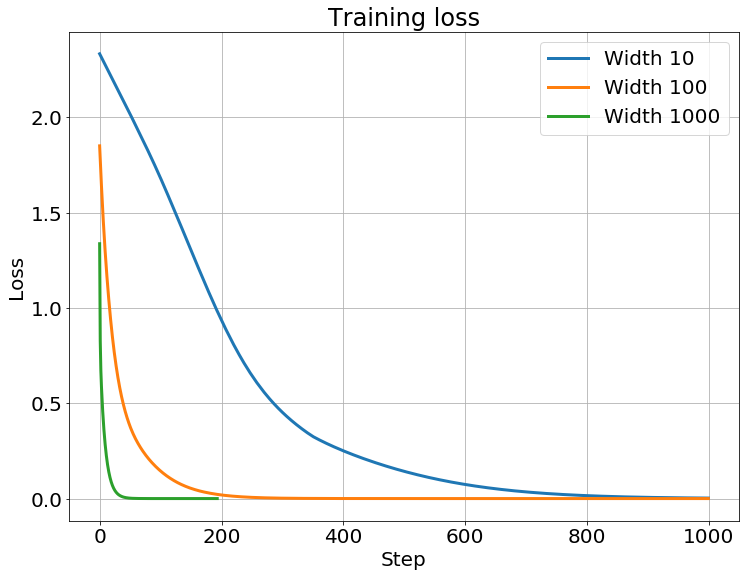
\includegraphics[width=.35\textwidth]{img/losses_3widths.png}
		\hspace{1em}
		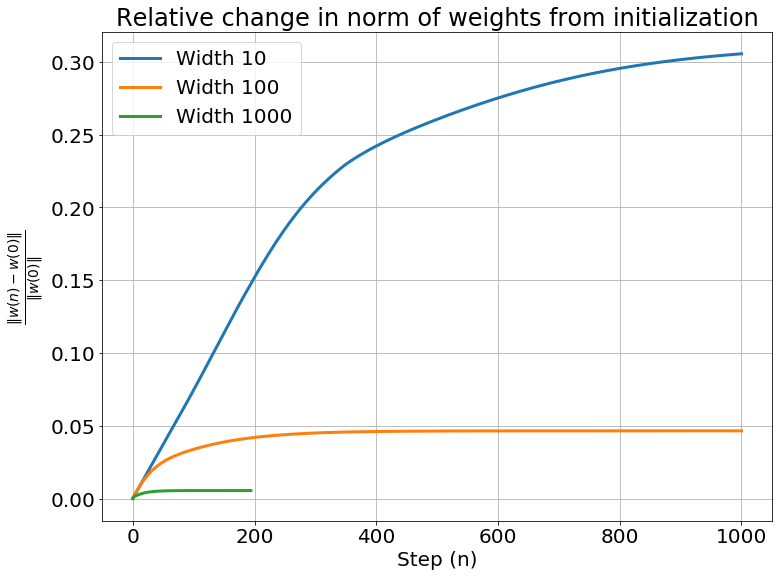
\includegraphics[width=.35\textwidth]{img/weightchange_3widths.png}
	\end{figure}
\end{frame}

\begin{frame}{Linear Approximation of $f_\theta$}
	Applying first-order taylor expansion of $f$ with respect to the evolution of parameters $\theta$, we have:
	\begin{gather}
		g_\theta (x) := f_{\theta_0}(x) + \langle \nabla_\theta f_{\theta_0}(x), \underbrace{\theta - \theta_0}_{\Delta \theta} \rangle
	\end{gather} \pause
	For convenience of analysis, we can set $\theta_0$ s.t.~$f_{\theta_0}(x) = 0~\forall x$. \pause Now,
	\begin{gather}
		g_\theta (x) := \langle \underbrace{\nabla_\theta f_{\theta_0}(x)}_{\phi(x)}, \Delta \theta  \rangle
	\end{gather} \pause
	Since we are in the overparameterized lazy learning regime, we have $\theta \approx \theta_0$, and $g_\theta \approx f_\theta$, which means:
	\begin{gather}
		\mathcal{L}(f_\theta, \mathcal{D}) \approx \mathcal{L}(g_\theta, \mathcal{D})
	\end{gather} \pause
	Now for $G^{(L)}: \mathbb{R}^p \rightarrow \mathcal{G}$ cost-composition $C \circ G^{L}: \mathbb{R}^p \rightarrow \mathbb{R}$ is convex!!
\end{frame}

\begin{frame}{Connection to Convergence}
	Next, notice $\phi(x)$ \textbf{does not} depend on post training parameters. \pause \newline \\

	We can use this to define feature map $\Phi$ over the entire dataset:
	\begin{gather}
		\Phi =
		\begin{bmatrix}
			\phi(x_i)^T
		\end{bmatrix}_n =
		\begin{bmatrix}
			\nabla f_{\theta_0}(x_i)^T
		\end{bmatrix}_n \in \mathbb{R}^{n \times p}
	\end{gather} \pause
	Optimizing $\mathcal{L}(f_\theta) \approx \text{optimizing } \mathcal{L}(g_\theta)$ which is convex in parameter space. \\
	So this is basically just linear regression:
	\begin{gather}
		\min_{g_\theta} \| y - g_\theta(x) \|^2_2 = 
		\min_{\Delta \theta} \|  y - \Phi \cdot \Delta \theta \|^2_2
	\end{gather}
	Comparing in output space, we can show that decay of error is exponential. \pause \newline \\
	
	\textbf{Caveat:} We're discussing gradient descent, not \textit{stochastic} gradient descent. In practice, we see performance dropoffs when optimizing over $g_\theta$.
\end{frame}

\begin{frame}{Defining NTK}
	We can define a kernel using our feature map $\phi$:
	\begin{gather}
		\kappa(x, x') = \phi(x)^T \phi(x') = \langle \nabla_\theta f_{\theta_0}(x), \nabla_\theta f_{\theta_0}(x') \rangle
	\end{gather}
	This kernel is the \textbf{neural tangent kernel}. \pause \newline \\

	The NTK effectively exists as part of gradient descent:
	\begin{gather}
		\theta_{t+1} = \theta_t - \nabla_\theta \mathcal{L}(f_{\theta_t}, \mathcal{D}) \\
		\frac{\partial \theta}{\partial t} = - \eta \nabla_\theta \mathcal{L}(\theta, \mathcal{D}) = - \frac{\eta}{n} \sum^n_{i=1} \nabla_\theta f_\theta(x_i) \nabla_{f_\theta} \ell(f_\theta, y_i) \\
		\frac{\partial f_\theta(x)}{\partial t} = \frac{\partial f_\theta(x)}{\partial \theta} \frac{\partial \theta}{\partial t} = - \frac{\eta}{n} \sum^n_{i=1} \underbrace{\nabla_\theta f_\theta(x) \nabla_\theta f_\theta(x_i)}_{NTK} \nabla_{f_\theta} \ell(f_\theta, y_i)
	\end{gather} \pause
	The NTK depends on $\theta_0$, is random at initialization and varies during training, but in the limit, this changes.
\end{frame}

\begin{frame}{Limiting Behavior of NTK}
	When the width tends to infinity, the NTK is deterministic at intitialization and doesn't change through training:
	\begin{gather}
		k \rightarrow \infty \implies f_{\theta,k} \rightarrow \mathcal{N}(0, \Sigma_k)~\forall k \in \{1, \ldots, n_L\}
	\end{gather} \pause
	Where covariance matrices $\Sigma_k$ are defined recursively as follows:
	\begin{align}
		\Sigma_1(x, x') &= \frac{1}{n_0} x^T x' + \beta^2 \\
		\Sigma_{k+1}(x, x') &= \mathbb{E}_{f \sim \mathcal{N}(0, \Sigma_k)}[\sigma(f(x)) \sigma(f(x'))] + \beta^2
	\end{align} \pause
	Which we further defines the limiting NTK:
	\begin{align}
		\kappa_1(x, x') &= \Sigma_1(x, x') \\
		\kappa_{k+1}(x, x') &= \kappa_{k}(x, x') \Sigma'_{k+1}(x, x') + \Sigma_k(x, x') \\
		\Sigma'_{k+1}(x, x') &= \mathbb{E}_{f \sim \mathcal{N}(0, \Sigma_k)}[\sigma'(f(x)) \sigma'(f(x'))] + \beta^2
	\end{align}
	Which is \underline{independent of initialization}.
\end{frame}

\begin{frame}{Training within the NTK Regime}
	During training $f_\theta$ follows a descent along the negative kernel gradient:
	\begin{gather}
		\partial_t f_{\theta_t} = -\nabla_{\Phi_{(L)}} C_{| f_{\theta_t}}
	\end{gather}

	% Training dynamics become an ODE and can be solved in closed form: 

	The Limiting Kernel is always \textit{positive definite}. By performing an eigendecomposition, we can decouple the gradient flow into eigenvectors, that decay at the rate of their eigenvalues. \pause \newline \\

	Since they all decay, NTK guaranteees that infinite width neural networks converge to a global minimum when trained to minimize empirical loss. \pause \newline \\

	\textbf{Bonus:} We have theoretical motivations for early-stopping; once the $k$ largest eigenvectors decay beyond a set threshold, stop training. \pause \newline \\

	\textbf{Caveat:} Computing NTK is expensive $\Omega(n^2)$ while regular GD uses $\mathcal{O}(d)$ samples.
\end{frame}

\begin{frame}{Thank you!}
	\begin{center}
		Have an awesome rest of your day!
	\end{center}
	\begin{center}
		\textbf{Slides:} \url{https://jinen.setpal.net/slides/ntk.pdf}
	\end{center}

	\textbf{References}:
	\begin{enumerate}[label=\arabic*.]
		\item Dwaraknath, Rajat. (Nov 2019). Understanding the Neural Tangent Kernel. \url{https://www.eigentales.com/NTK/}
		\item Ma, Tengyu. (Nov 2022). Stanford CS229M - Lecture 13: Neural Tangent Kernel. \url{https://youtu.be/btphvvnad0A}
		\item Ma, Tengyu. (Nov 2022). Stanford CS229M - Lecture 14: Neural Tangent Kernel, Implicit regularization of gradient descent. \url{https://youtu.be/xpT1ymwCk9w}
		\item Weng, Lilian. (Sep 2022). Some math behind neural tangent kernel. \url{https://lilianweng.github.io/posts/2022-09-08-ntk/}
		\item Pietraho, Thomas. Math 2805: Mathematical principles of machine learning. {\small\url{https://web.bowdoin.edu/~tpietrah/hugo/math2805/docs/unsupervised_learning/dim_reduction/hw_operator_norms/}}
	\end{enumerate}
\end{frame}

\end{document}
